\documentclass[unicode,a4paper,10pt]{ltjsarticle}
% ---fonts---
\PassOptionsToPackage{quiet}{fontspec}
\usepackage{luatexja-fontspec}
\setmainfont{TeX Gyre Termes}
\setmainjfont[BoldFont = IPAGothic]{IPAMincho}
% \setmainjfont{Noto Sans CJK JP}
\setmathrm{Latin Modern Roman}

% ---Display \subsubsection at the Index
% \setcounter{tocdepth}{3}

% ---Setting about the geometry of the document----
% \usepackage{a4wide}
% \pagestyle{empty}

% ---Physics and Math Packages---
\usepackage{amssymb,amsfonts,amsthm,mathtools}
\usepackage{physics,braket,bm}

% ---underline---
\usepackage[normalem]{ulem}

% ---cancel---
\usepackage{cancel}

% --- surround the texts or equations
% \usepackage{fancybox,ascmac}

% ---settings of theorem environment---
\theoremstyle{definition}
\newtheorem{dfn}{定義}
\newtheorem{prop}{命題}
\newtheorem{thm}{定理}
\newtheorem{exm}{例}
\newtheorem{exc}{演習}

% ---settings of proof environment---
\renewcommand{\proofname}{\textbf{証明}}
\renewcommand{\qedsymbol}{$\blacksquare$}

% ---Ignore the Warnings---
\usepackage{silence}
\WarningFilter{latexfont}{Some font shapes}
\WarningFilter{latexfont}{Font shape}
\WarningFilter{latexfont}{Size substitutions}
\ExplSyntaxOn
\msg_redirect_name:nnn{hooks}{generic-deprecated}{none}
\ExplSyntaxOff

% ---Insert the figure (If insert the `draft' at the option, the process becomes faster.)---
\usepackage{graphicx}
% \usepackage{subcaption}

% ----Add a link to a text---
\usepackage{url,hyperref}
\usepackage[dvipsnames,svgnames]{xcolor}
\hypersetup{colorlinks=true,citecolor=FireBrick,linkcolor=Navy,urlcolor=purple}
% ---refer `texdoc xcolor' at the command line---

% ---Tikz---
% \usepackage{tikz,pgf,pgfplots,circuitikz}
% \pgfplotsset{compat=1.15}
% \usetikzlibrary{intersections,arrows.meta,angles,calc,3d,decorations.pathmorphing}

% ---Add the section number to the equation, figure, and table number---
\makeatletter
   \renewcommand{\theequation}{$\thesection.\arabic{equation}$}
   \@addtoreset{equation}{section}
   
   \renewcommand{\thefigure}{\thesection.\arabic{figure}}
   \@addtoreset{figure}{section}
   
   \renewcommand{\thetable}{\thesection.\arabic{table}}
   \@addtoreset{table}{section}
\makeatother

% ---enumerate---
% \renewcommand{\labelenumi}{$\arabic{enumi}.$}
% \renewcommand{\labelenumii}{$(\arabic{enumii})$}

% ---Index---
% \usepackage{makeidx}
% \makeindex 

% ---Title---
\title{
  title
}
\author{
  author
}
\date{最終更新:\today}

\begin{document}

% ---Title---
\title{
  素粒子物理学\ 中間レポート
}
\author{
  学生番号:5324A057-8
  \quad
  氏名:宮根 一樹
}
\date{最終更新:\today}

\maketitle

\begin{enumerate}
  \item
        与えられたラグランジアンは
        \begin{equation}
          \mathcal{L}
          =
          \bar{\psi}^{\alpha}(i\gamma^{\mu}\partial_{\mu}-m_{f})_{\alpha}^{\ \beta}\psi_{\beta}
          +
          \frac{1}{2}(\partial_{\mu}\phi)^2
          -
          \frac{1}{2}m_{\phi}^2\phi^2
          +
          Y\phi\bar{\psi}\psi
          。
        \end{equation}
        ただし、$\alpha,\beta$はガンマ行列$\gamma^{\mu}$の成分の添え字である。したがって、
        \begin{equation}
          \left\{
          \begin{alignedat}{1}
            \pdv{\mathcal{L}}{\bar{\psi}^{\xi}}
            &=
            i(\gamma^{\mu}\partial_{\mu}-m_{f})_{\xi}^{\ \eta}\psi_{\eta}(x)
            +
            Y\phi(x)\psi_{\xi}(x)
            、
            \\
            \pdv{\mathcal{L}}{(\partial_{\mu}\bar{\psi}^{\xi})}
            &=
            0
            、
            \\
            \pdv{\mathcal{L}}{\phi}
            &=
            -
            m_{\phi}^2\phi+Y\bar{\psi}\psi
            、
            \\
            \pdv{\mathcal{L}}{(\partial_{\mu}\phi)}
            &=
            \partial^{\mu}\phi
          \end{alignedat}
          \right.
        \end{equation}
        となっているので、オイラー・ラグランジュ方程式から運動方程式
        \begin{graybox}

          \vspace*{-10pt}

          \begin{gather}
            (i\gamma^{\mu}\partial_{\mu}-m_{f})_{\xi}^{\ \eta}\psi_{\eta}(x)
            =
            -Y\phi(x)\psi_{\xi}(x)
            、
            \\
            (\partial_{\mu}\partial^{\mu}+m_{\phi}^{2})\phi(x)
            =
            Y\bar{\psi}^{\xi}(x)\psi_{\xi}(x)
          \end{gather}
        \end{graybox}
        が得られる。


  \item
        $\gamma^{\mu}\partial_{\mu}=\gamma^{0}\partial_{0}+\gamma^{i}\partial_{i}$であることに注意して、運動方程式の項を整理すると
        \begin{equation}
          i\gamma^{0}\partial_{0}\psi(x)
          =
          (-i\gamma^{i}\partial_{i}+m_{f}-Y\phi)\psi(x)
        \end{equation}
        となる。ただし、イタリックの添え字$i$は空間方向の添え字$i=1,2,3$である。ここで、両辺に左側から$\gamma^{0}$をかけると、${\gamma^{0}}^2=1$であるから
        \begin{equation}
          i\partial_{0}\psi
          =
          (
          \uline{-i\gamma^{0}\gamma^{i}\partial_{i}
          +
          \gamma^{0}m_{f}
          }
          \uwave{
            -
            \gamma^{0}Y\phi(x)
          }
          )\psi(x)
        \end{equation}
        となる。したがって、\uline{下線の項}を$H_{0}$、\uwave{波線の項}を$V(x)$とすれば、
        \begin{equation}
          i\partial_{0}\psi
          =
          (
          H_{0}
          +
          V(x)
          )\psi(x)
        \end{equation}
        であり、確かに$V(x)=-\gamma^{0}V(x)$となっている。


  \item
        図\ref{fig:feynman_diag01}の値を計算する。遷移振幅に具体的な表式を代入すると
        \begin{align}
          iT_{\textrm{FI}}
           & =
          -iY
          \int\dd^4 x\
          \bar{\psi}_{\textrm{F}}(x)\phi(x)\psi_{\textrm{I}}(x)
          \nonumber
          \\
           & =
          iY
          \int\dd^4 x\
          \bar{u}(\bm{q}_{1},\tau_{1})u(\bm{p}_{1},\lambda_{1})e^{-i(p_{1}-q_{1})\cdot x}
          \times
          \phi(k)e^{-ik\cdot x}
          \label{eqn:hogehoge}
        \end{align}
        となる。ここで、クライン・ゴルドン方程式
        \begin{equation}
          (\partial^2+m_{\phi})\phi(x)
          =
          Y\bar{\psi}\psi
        \end{equation}
        に展開式を代入すると
        \begin{gather}
          (-k^2+m_{\phi}^2)\phi(k)e^{-ik\cdot x}
          =
          Y\bar{u}(\bm{q}_{2},\tau_{2})u(\bm{p}_{2},\lambda_{2})
          \times
          e^{-i(p_{2}-q_{2})\cdot x}
        \end{gather}
        となるので、これを\eqref{eqn:hogehoge}に代入すれば
        \begin{graybox}

          \vspace*{-10pt}

          \begin{align}
            iT_{\textrm{FI}}
             & =
            iY
            \int\dd^4 x\
            \bar{u}(\bm{q}_{1},\tau_{1})u(\bm{p}_{1},\lambda_{1})
            \left.\dfrac{i^2 Y}{k^2-m_{\phi}^2}\right|_{k=p_{1}-q_{1}}
            \bar{u}(\bm{q}_{2},\tau_{2})u(\bm{p}_{2},\lambda_{2})
            e^{-i(p_{1}-q_{1}+p_{2}-q_{2})\cdot x}
            \nonumber
            \\
             & =
            (2\pi)^4\delta^{(4)}(p_{1}-q_{1}+p_{2}-q_{2})
            \nonumber
            \\
            &\hspace*{1cm}
            \times
            i(iY)^2
            \bar{u}(\bm{q}_{1},\tau_{1})u(\bm{p}_{1},\lambda_{1})
            \left.\dfrac{i}{k^2-m_{\phi}^2}\right|_{k=p_{1}-q_{1}}
            \bar{u}(\bm{q}_{2},\tau_{2})u(\bm{p}_{2},\lambda_{2})
          \end{align}
          となるので、
          \begin{equation}
            \mathcal{M}
            =
            (iY)^2
            \bar{u}(\bm{q}_{1},\tau_{1})u(\bm{p}_{1},\lambda_{1})
            \left.\dfrac{i}{k^2-m_{\phi}^2}\right|_{k=p_{1}-q_{1}}
            \bar{u}(\bm{q}_{2},\tau_{2})u(\bm{p}_{2},\lambda_{2})
          \end{equation}
        \end{graybox}
        である\footnote{
          ただし、運動量保存則から$k=p_{1}-q_{1}$であることを暗に用いている。
          }。

        \begin{figure}[ht]
          \centering
          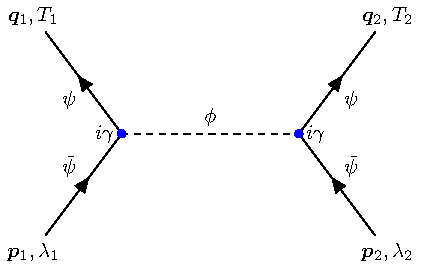
\includegraphics[width=0.6\textwidth]{fig/fig01.pdf}
          \caption{問題のダイアグラム}
          \label{fig:feynman_diag01}
        \end{figure}


  \item
        非相対論的極限では、$(p_{1}-q_{1})^2\sim -|\bm{p}_{1}-\bm{q}_{1}|^2$が成立している。よって、プロパゲーターは
        \begin{equation}
          \left.\dfrac{i}{k^2-m_{\phi}^2}\right|_{k=p_{1}-q_{1}}
          \sim          
          \dfrac{-i}{|\bm{p}_{1}-\bm{q}_{1}|^2+m_{\phi}^2}
        \end{equation}





\end{enumerate}


\clearpage
\uline{補足}
\begin{enumerate}
  \item
        ここで、問2で仮定した
        \begin{equation}
          H_{0}
          =
          -i\gamma^{0}\gamma^{i}\partial_{i}+\gamma^{0}m_{f}
        \end{equation}
        が、今回のディラック場の理論のハミルトニアンであることを確認しておこう。そのためには、$\psi$に共役な運動量をもとめればよい。それは
        \begin{equation}
          \pi_{\psi}
          =
          \pdv{\mathcal{L}}{(\psi_{0}\psi)}
          =
          \bar{\psi}i\gamma^{0}
          =
          i\psi^{\dag}
        \end{equation}
        であるので、自由ディラック場をルジャンドル変換をすれば
        \begin{align}
          H_{0}
           & =
          \pi_{\psi}\partial_{0}\psi
          -
          \mathcal{L}_{\textrm{Dirac}}
          \nonumber
          \\
           & =
          \psi^{\dag}(-i\gamma^{0}\gamma^{i}\partial_{i}+\gamma^{0}m_{f})\psi
        \end{align}
        となるため、ハミルトニアンが得られる。

\end{enumerate}

% ----------------------------------------
% \clearpage
% \bibliography{ref}
% \bibliographystyle{ytphys}

\end{document}
